\documentclass[table,serif,mathserif,final]{beamer}
\mode<presentation>{\usetheme{Lankton}}
\RequirePackage{ragged2e}
\usepackage{amsmath,amsfonts,amssymb,pxfonts,xspace}
\usepackage{graphicx}
\graphicspath{{./figures/}}
\usepackage[orientation=landscape,size=custom,width=121.92,height=121.92,scale=.5,debug]{beamerposter}
%\usepackage{pslatex} % use times roman
\usepackage{amsmath}
\usepackage{amssymb}
\usepackage{amsthm}
\usepackage{color}
\usepackage{array}
\usepackage{xy}
\usepackage{setspace}
\usepackage{tikz}
\usetikzlibrary{matrix}
\usepackage{mathptmx }
\usetikzlibrary{arrows,shapes}
\usepackage{pifont}
\newcommand{\cmark}{{\color{blue}\fontsize{65}{60}\selectfont \ding{51}}}%
\newcommand{\xmark}{{\color{red}\fontsize{65}{60}\selectfont \ding{55}}}%
\newcommand{\citefont}[1]{{\huge \textcolor{gray}{#1}}}


\usepackage[makeroom]{cancel}
\usepackage{verbatim}
\usetikzlibrary{arrows,shapes}

\usepackage{algorithm, algpseudocode}
\def\E{\operatorname{\mathbb{E}}}
\newcommand{\polylog}{\operatorname{polylog}}
\newcommand{\poly}{\operatorname{poly}}

\newcommand*\mycirc[1]{%
  \begin{tikzpicture}
    \node[draw,circle,inner sep=1pt] {#1};
  \end{tikzpicture}}

\newcommand\iitem{\item[\begin{Large}$\bullet$\end{Large}]}

\newcommand{\rot}{\operatorname*{rot}}

%\usepackage[pdftex]{graphicx}
%\usepackage[left=1.5in,right=1.5in, top=1.5in,bottom=1.5in,]{geometry}
\newcommand{\edit}[1]{{\color{red}\textbf{#1}}}
\newcommand{\CC}{\mathbb{C}}
\newcommand{\NN}{\mathbb{N}}
\newcommand{\ZZ}{\mathbb{Z}}
\newcommand{\ot}{\otimes}
\newcommand{\sign}{\operatorname{sign}}

%----------------MACROS---------------%
\newtheorem{thm}{Theorem}[section]
\newtheorem{defn}[thm]{Definition}
\newtheorem{lem}[thm]{Lemma}
\newtheorem{prop}[thm]{Proposition}
\newtheorem{clm}[thm]{Claim} 
\newtheorem{cor}[thm]{Corollary}
\newtheorem{conj}[thm]{Conjecture}
\theoremstyle{remark}
\newtheorem{rem}[thm]{Remark}
\newtheorem{ex}[thm]{Example}

\newcommand{\mycenter}[1]{\hfil #1 \hfil}
\newcommand{\myzero}{\hfil $0$ \hfil}
\newcommand{\ca}{\cellcolor{ca}}
\newcommand{\cb}{\cellcolor{cb}}
\newcommand{\cc}{\cellcolor{cc}}
\def \av {\text{AV}}
\newcommand{\match}[3]{
\item {\textbf{#1}\newline Appears for #2 sets of patterns. \\ Example match: $\av_n($#3$)$ }
}
\newcommand{\matchone}[2]{
\item {\textbf{#1}\newline Match: #2 \newline}
}

\newcommand{\footleft}{}
\newcommand{\footright}{}
%% %\dologotrue
\title{Cache Efficient Parallel Partition Algorithms \\An In-Place Exclusive Read/Write Memory Algorithm}

%-- Header and footer information ----------------------------------
\setbeamertemplate{headline}{
 \leavevmode
    \vskip1cm
    \centering
    \usebeamercolor{title in headline}{\fontsize{40}{50}\selectfont \textbf{\inserttitle} \\[0.5ex]}
    % \usebeamercolor{author in headline}{\Huge{\insertauthor}\\[1ex]}
    % \usebeamercolor{institute in headline}{\Huge{\insertinstitute}\\[1ex]}

 \hspace{0.5in}\begin{beamercolorbox}[wd=47in,colsep=0.15cm]{cboxb}\end{beamercolorbox}
}


%-------------------------------------------------------------------
\definecolor{math}{rgb}{0.4,0.4,1}
%\definecolor{proven}{rgb}{0.4,0.4,1}
%\definecolor{conject}{rgb}{0.7.0,7,1}
%\definecolor{comput}{rgb}{09,0.9,1}
%\definecolor{lightslateblue}{rgb}{0.517647,0.43921569,1} % light slate blue 0x8470ff (132,112,255)
%\definecolor{proven}{rgb}{0.52941176,0.80784313,0.98039} % sky blue 0x87ceeb (135,206,250)
%\definecolor{conject}{rgb}{0.7.0,7,1}
%\definecolor{comput}{rgb}{0.9,0.9,1}
%\definecolor{proven}{rgb}{0.7,1,1} % sky blue 0x87ceeb (135,206,250)
%\definecolor{conject}{rgb}{0.4,0.4,1}
%\definecolor{comput}{rgb}{1,0.9,1}

%\definecolor{proven}{rgb}{0.59608,0.98431,0.59608} % pale green 0x98fb98 152,251,152
%\definecolor{comput}{rgb}{0.75,1,0.75} % pale green 0x98fb98 152,251,152
\definecolor{ca}{rgb}{0.875,1,0.875} % lighter than pale green
\definecolor{cb}{rgb}{0.75,1,1} % sky blue 0x87ceeb (135,206,250)
\definecolor{cc}{rgb}{1,0.9,1}
%\definecolor{comput}{rgb}{1,1,1} % sky blue 0x87ceeb (135,206,250)


\definecolor{darkgreen}{rgb}{0.4,0.8,0.5} 

%-- Main Document --------------------------------------------------
\begin{document}
\begin{frame}{}
\begin{columns}[t]
\begin{column}{0.02\linewidth}
\end{column}

\begin{column}{0.21\linewidth}

\begin{block}{\Huge What is The Partition Problem?}
  \justifying
  \Huge
  \textbf{Explanation:} The \emph{Partition Problem} is to reorder the elements in a list so that elements in the same group occur in the same part of the list.

  \textbf{Example:} A common way of grouping elements is based on whether they exceed or fall short of a certain ``pivot" value.

  {\color{blue} An unpartitioned array:}

  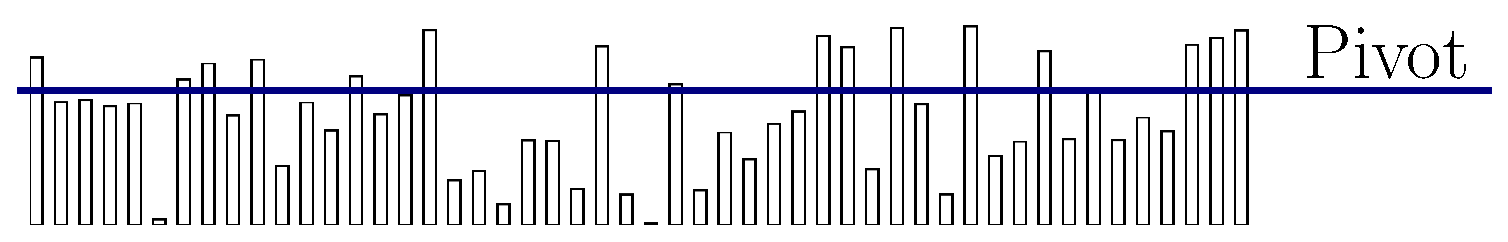
\includegraphics[width=\linewidth]{imgs/partitionDefn/partitionDefn1Ann.eps}
  {\color{blue} An array partitioned relative to the pivot value:}

  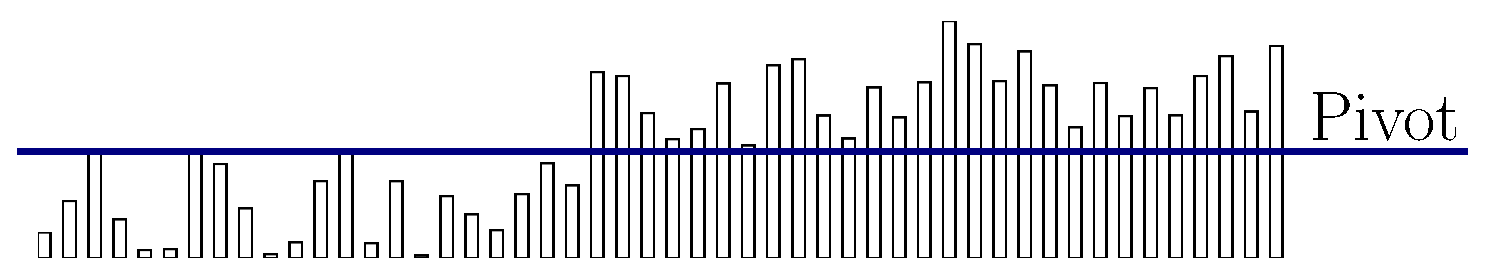
\includegraphics[width=\linewidth]{imgs/partitionDefn/partitionDefn2Ann.eps}
\end{block}
\vspace{0.5cm}

\begin{block}{\Huge What is A Parallel Algorithm?}
  \justifying
  \Huge
  \textbf{Explanation:} Whereas a typical (i.e. serial) algorithm runs on a
  single processor, a \emph{parallel algorithm} runs on $p \geq 1$ processors.\\
  In our model of parallelism, we only allow the concurrency mechanism of
  parallel-for-loops; in particular our algorithm doesn't make concurrent
  writes to data (it is \textbf{EREW}): we don't allow locks or atomic variables. Being
  EREW is desirable because theoretical predictions apply more readily to them,
  and because EREW algorithms are hardware independent. %, unlike some programs utilizing atomic variables for instance.

  \textbf{Example:} Many tasks have parts that can be performed concurrently; such tasks can be performed faster with parallel computing.

  {\color{blue} Program execution in serial and in parallel: }

  \centering
  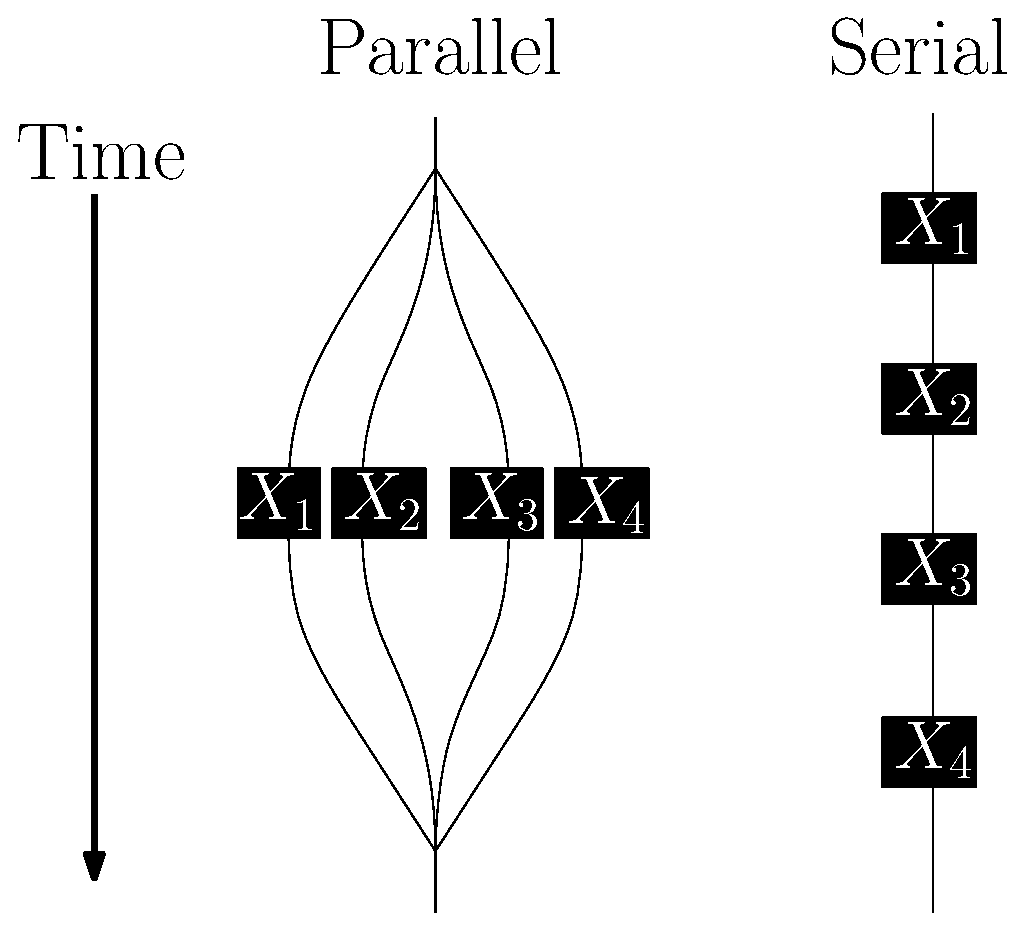
\includegraphics[width=0.6\linewidth]{imgs/parallelForLoop/serialParallelComparison.eps}
\end{block}
\vspace{0.5cm}

\begin{block}{\Huge Performance Metrics for Parallel Algorithms}
  \Huge
  \begin{columns}[T]
    \begin{column}{0.5\linewidth}
    \begin{figure}
      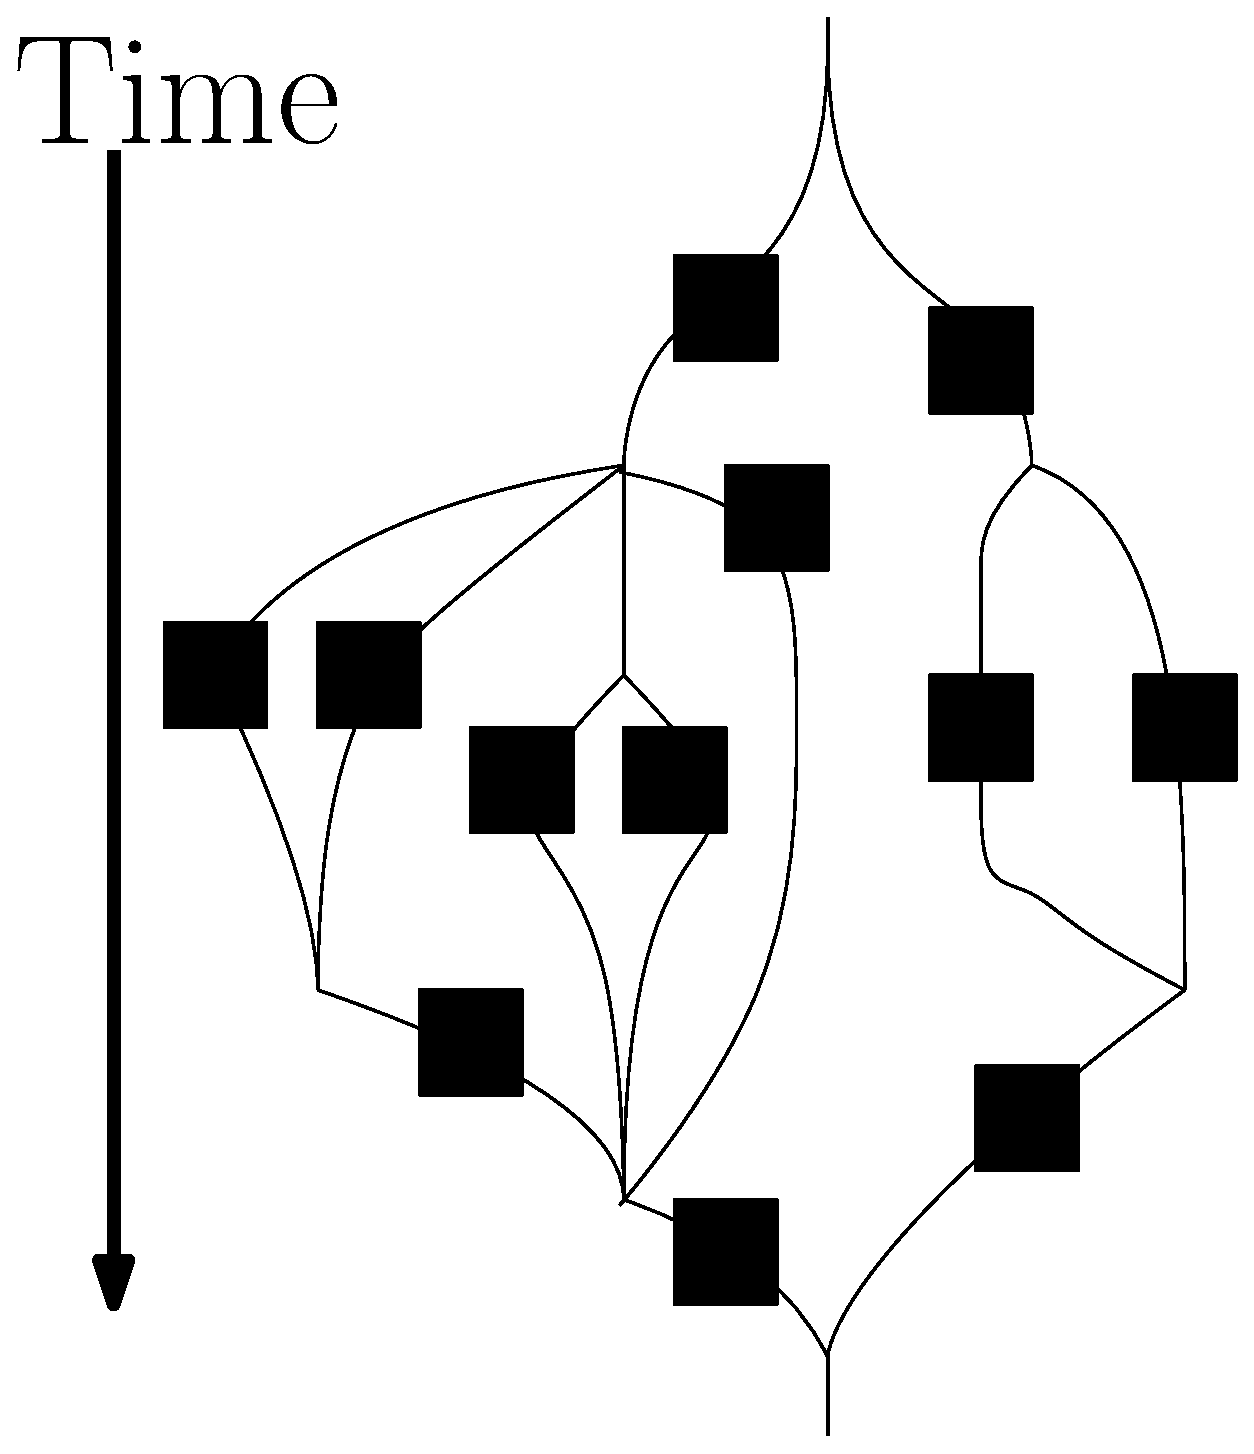
\includegraphics[width=0.8\linewidth]{imgs/parallelForLoop/altParallelForLoopComposition.eps}
    \end{figure}
    \end{column}
    \hfill
    \begin{column}{0.5\linewidth}
    Important extreme cases:\\
    \vspace{0.3cm}
    \textbf{Work:} $T_1$
    \begin{itemize}
      \item time to run in serial
      \item "sum of all work"
    \end{itemize}
    \vspace{0.3cm}
    \textbf{Span:} $T_\infty$
    \begin{itemize}
      \item time to run on infinitely \\many processors
      \item "height of the graph"
    \end{itemize}	
    \end{column}
\end{columns}
\end{block}
\vspace{0.5cm}

\begin{block}{\Huge What is Cache Efficiency?}
  \justifying
  \Huge
  \textbf{Explanation:} \emph{Cache} is a small part of memory that can be accessed much faster than ordinary RAM. When data is already loaded into Cache a program can rapidly access it; this is called a \emph{cache hit}. When data needed by a program isn't in cache it must be loaded into cache; this is called a \emph{cache miss}, and takes time. \\
  \textbf{Remark:} An algorithm with very few cache misses is \emph{Cache Efficient}; cache efficiency leads to faster performance in practice.\\
  \textbf{Factors in Cache-Efficiency:}
  \begin{itemize}
    \item Perform low number of passes over the data
    \item Don't use extra memory, i.e. are \emph{In-Place}
    \item Deal with elements that are close in memory together
  \end{itemize}
\end{block}
\vspace{0.5cm}

\begin{block}{\Huge Previous Work on the Partition Problem}
  \justifying
  \Huge
  The ``Standard Algorithm" is {\color{darkgreen} theoretically optimal with span $O(\log n)$,} {\color{red} but slow in practice due to poor cache behavior.}

  The {\color{darkgreen}fastest algorithms in practice} {\color{red}lack theoretical guarantees}
  \begin{itemize}
    \item Lock-based and atomic-variable based algorithms\\ \citefont{[Michael Axtmann, Sascha Witt, Daniel Ferizovic, and Peter Sanders, 2017; Philip Heidelberger, Alan Norton, and John T. Robinson, 1990; Philippas Tsigas and Yi Zhang, 2003]}\\
      {\color{red} Not Exclusive Read/Write Memory}
    \item The Strided Algorithm\\ \citefont{[Francis and Pannan, 92; Frias and Petit, 08]}\\ 
      {\color{darkgreen}No locks or atomic-variables,} {\color{red}but no bound on span}
  \end{itemize}
\end{block}
\end{column}

\begin{column}{0.02\linewidth}
\end{column}

\begin{column}{0.2\linewidth}

\begin{block}{\Huge Why is The Partition Problem Important?}
  \justifying
  \Huge
  The Partition Problem is a fundamental problem in computer science. Additionally, it is a subproblem that must be solved in many algorithms such as:
  \begin{itemize}
    \item \emph{Parallel Quicksort} (the most famous and important application partition algorithms)
    \item \emph{Filtering operations}
  \end{itemize}
  Furthermore, the partition problem is of great practical importance as:
  \begin{itemize}
    \item Humans want organized data often, e.g. performing ``ORDER BY" on information from a database, or simply ordering data in a spreadsheet 
    \item Many algorithms run faster, or rely on, having sorted data 
  \end{itemize}
\end{block}
\vspace{0.5cm}

\begin{block}{\Huge Our Research Question}
  \justifying
  \Huge Can we create an algorithm with \emph{theoretical guarantees} that is \emph{fast in practice}?
\end{block}

\vspace{0.5cm}
\begin{block}{\Huge Result}
  \justifying
  \Huge We created the \emph{Smoothed Striding Algorithm}. \\
  Key Features:
	\begin{itemize}
		\item linear work and polylogarithmic span \\
			{\color{blue} (like the Standard Algorithm)\\}
		\vspace{0.15cm}
		\item fast in practice \\
			{\color{blue} (like the Strided Algorithm)\\}
	\vspace{0.15cm}
		\item theoretically optimal cache behavior \\
			{\color{blue} (unlike any past algorithm)}
	\end{itemize}
\end{block}

\vspace{0.5cm}
\begin{block}{\Huge Smoothed Striding Algorithm's Performance}
	\begin{figure}
		\begin{center}
			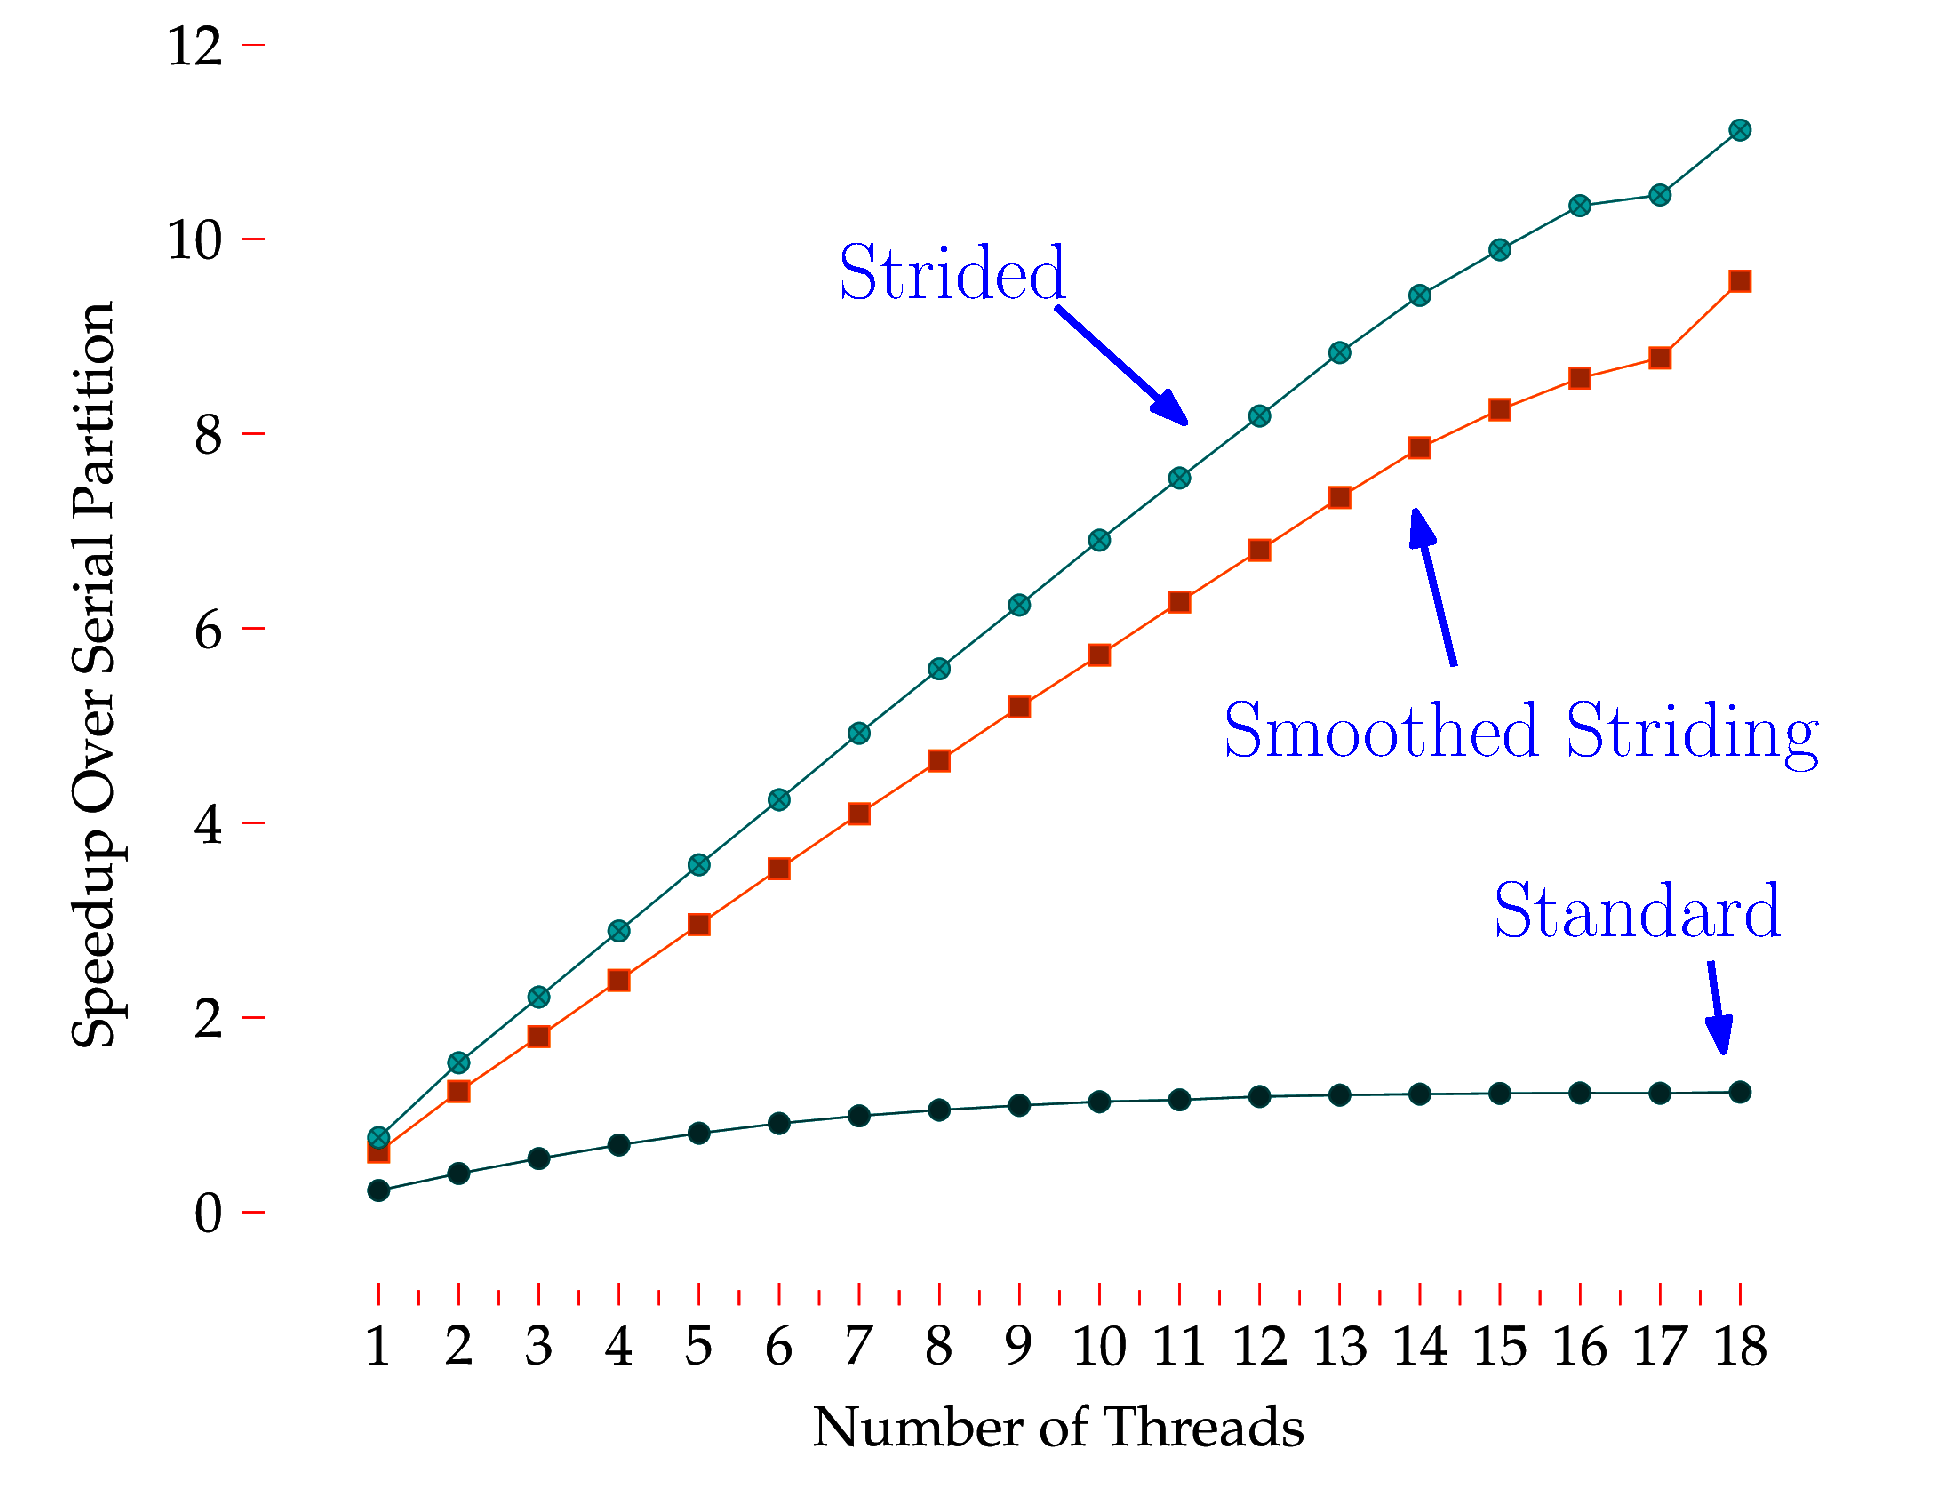
\includegraphics[width=0.9\linewidth]{imgs/compiledGraph.eps}
		\end{center}
	\end{figure}
\end{block}

\vspace{0.5cm}
\begin{block}{\Huge Strided Versus Smoothed-Striding Algorithm}
  \Huge
	\begin{columns}[T] % align columns
	\begin{column}{.4\textwidth}
		\textbf{Strided Algorithm}\\\citefont{[Francis and Pannan, 92; Frias and Petit, 08]}\\
		\vspace{0.25cm}
		\begin{itemize}
			\item Good cache behavior in practice\\\hfill
			\item Worst case span is $T_\infty \approx n$\\\hfill\\\hfill
			\item On random inputs span is $T_\infty = \tilde{O}(n^{2/3})$
		\end{itemize}
	\end{column}
	\hfill
	\begin{column}{.5\textwidth}
		\textbf{Smoothed-Striding Algorithm}\\\citefont{}\\
		\vspace{0.25cm}
		\begin{itemize}
			\item Provably optimal cache behavior\\\hfill
			\item Span is \\$T_\infty = O(\log n \log\log n)$\\ with high probability in $n$\\\hfill
			\item Uses randomization \emph{inside} the algorithm % both about the recursion step and the no worst case inputs thing
		\end{itemize}
	\end{column}
	\end{columns}

\end{block}

\vspace{0.5cm}
\begin{block}{\Huge Application To Parallel Quicksort}
  \Huge
  Parallel Quicksort is the most important application of Parallel Partition. Parallel Quicksort works as follows:

  \begin{itemize}
    \item Chose a pivot value randomly from the array
    \item \emph{Partition} the array relative to the pivot value 
    \item Recursively sort the subarrays (in parallel)
  \end{itemize}

  The depth of recursion is $O(\log n)$ with high probability in $n$, and each
  level of recursion requires span $O(\log n \log \log n)$ when using the
  Smoothed Striding algorithm. This results in span $O(\log^2 n \log \log n)$
  and work $O(n\log n)$ for the entire Parallel Quicksort -- which is
  within a factor of $\log \log n$ of optimal span -- while additionally guaranteeing
   cache-friendliness.

  \begin{center}
  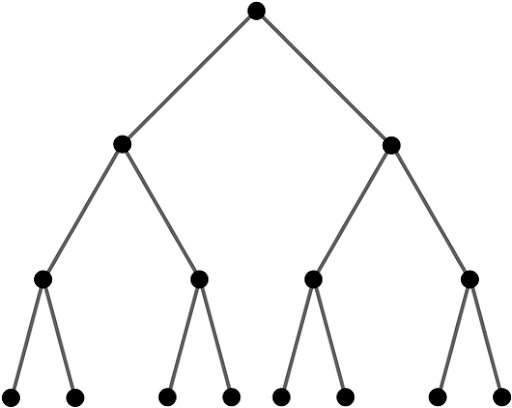
\includegraphics[width=0.45\linewidth]{imgs/tree.png}
  \end{center}
\end{block}

  \end{column}

\begin{column}{0.005\linewidth}
\end{column}
  \begin{column}{0.295\linewidth}
\begin{block}{\Huge Smoothed Striding Algorithm}
  \Huge
	Logically partition the array into chunks of adjacent elements.
	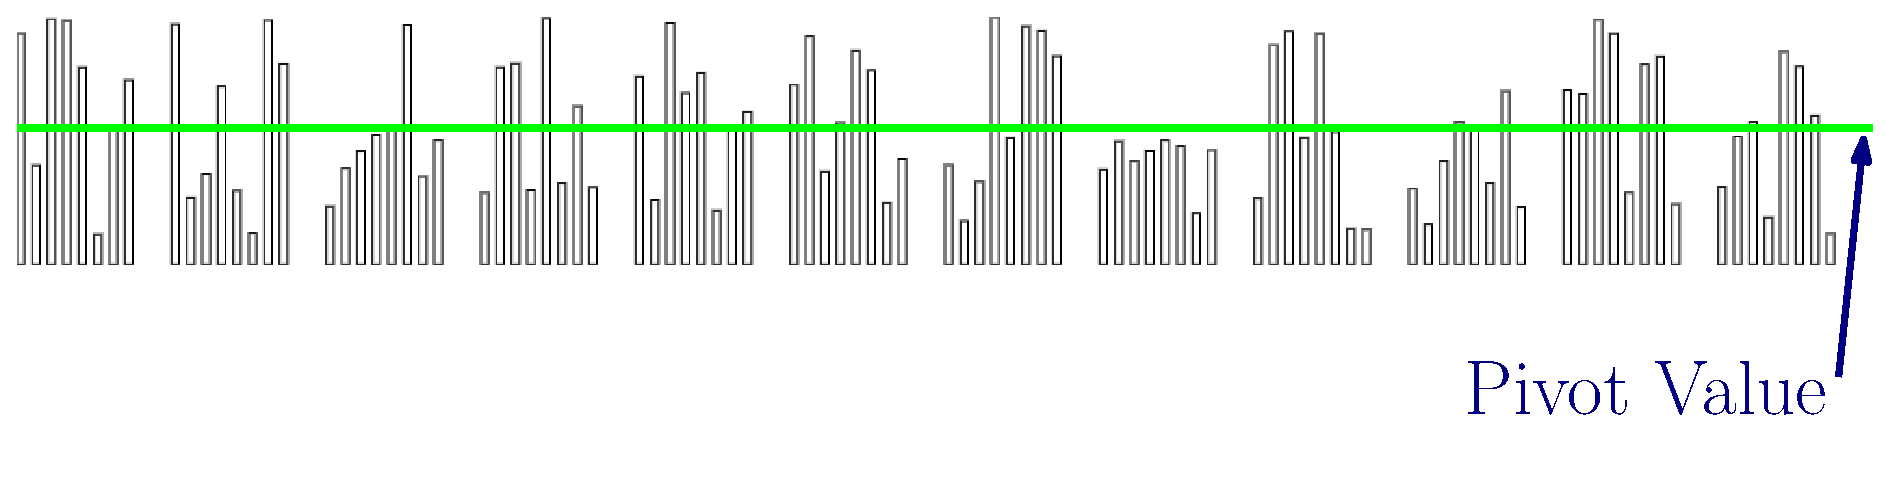
\includegraphics[width=\linewidth]{imgs/smoothedStridingAlgSim/sim1.eps}
	Form groups $U_i$ that contain a random element from each chunk. \\
  {\color{blue}This randomization step was one of our key insights; it guarantees that the $U_i$'s have similar compositions regardless of the input.}
	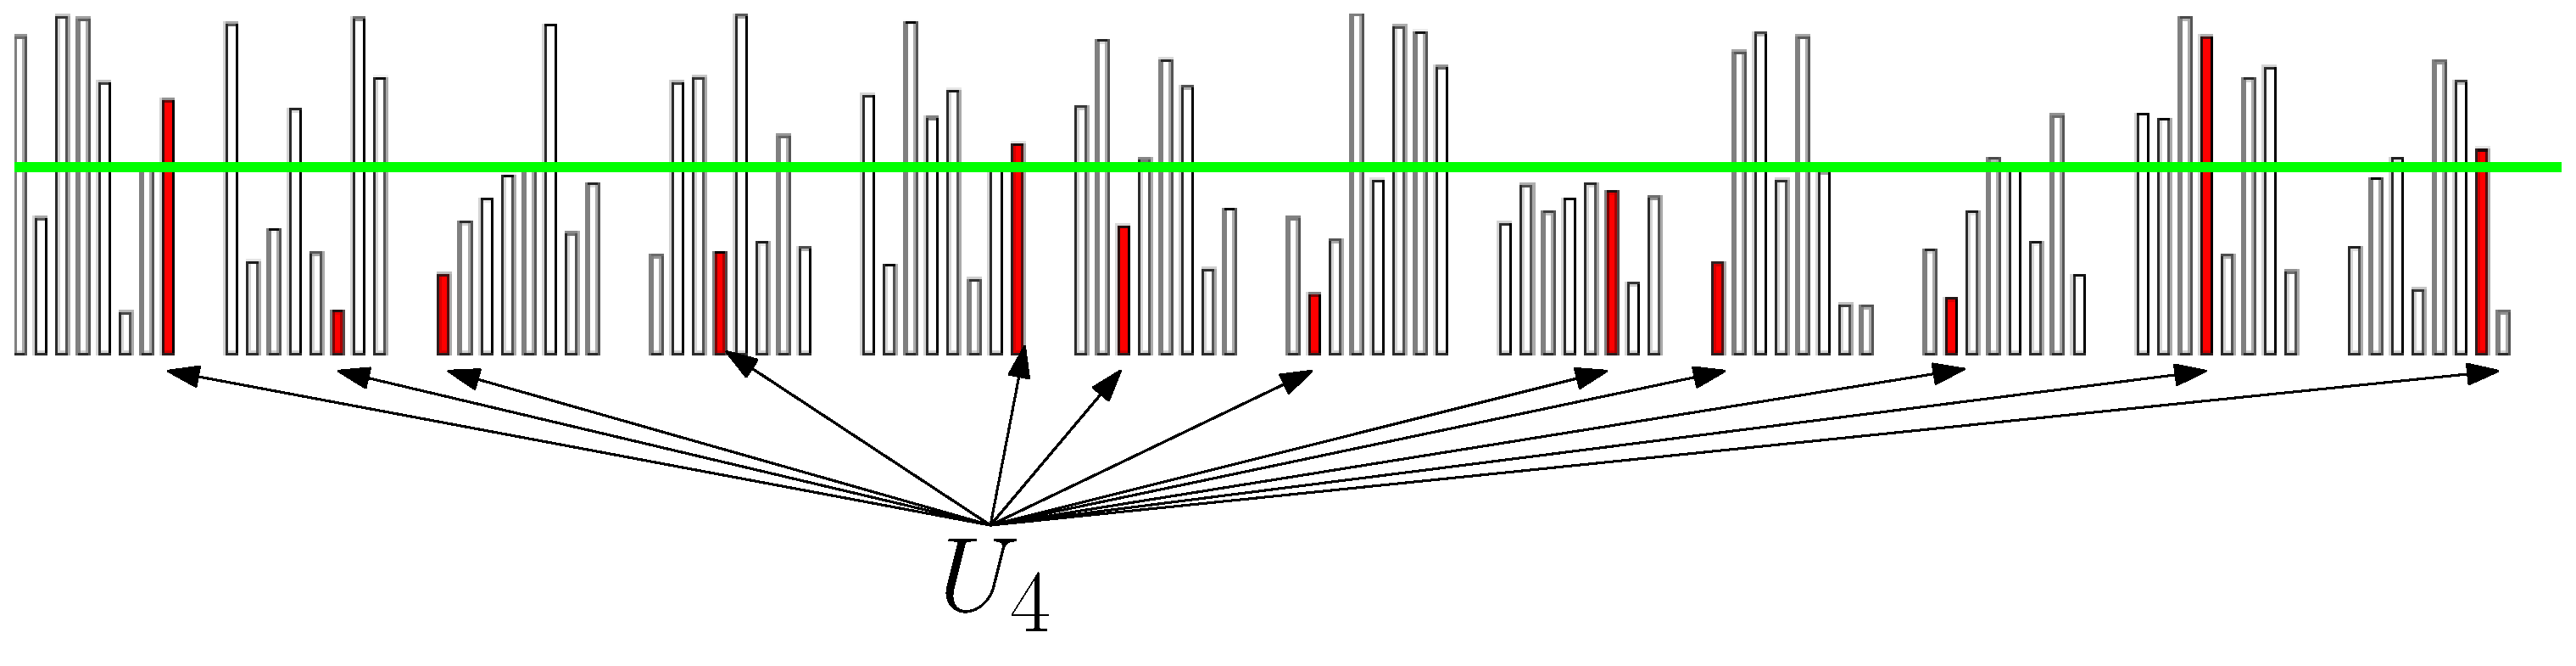
\includegraphics[width=\linewidth]{imgs/smoothedStridingAlgSim/sim2.eps}
	Perform serial partitions on each $U_i$ in parallel over the $U_i$'s. \\
  This step is highly parallel.
	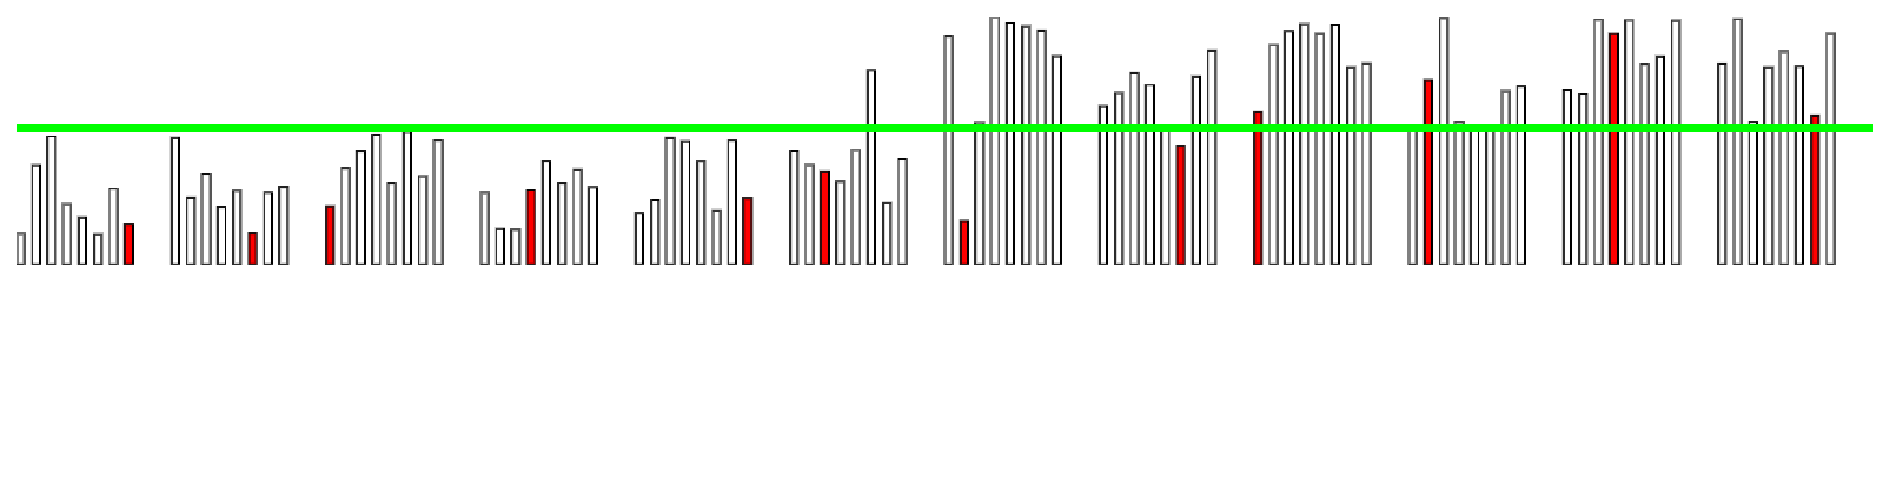
\includegraphics[width=\linewidth]{imgs/smoothedStridingAlgSim/sim3.eps}
  Define $v_i = $ index of first element greater than the pivot in $U_i$. 
	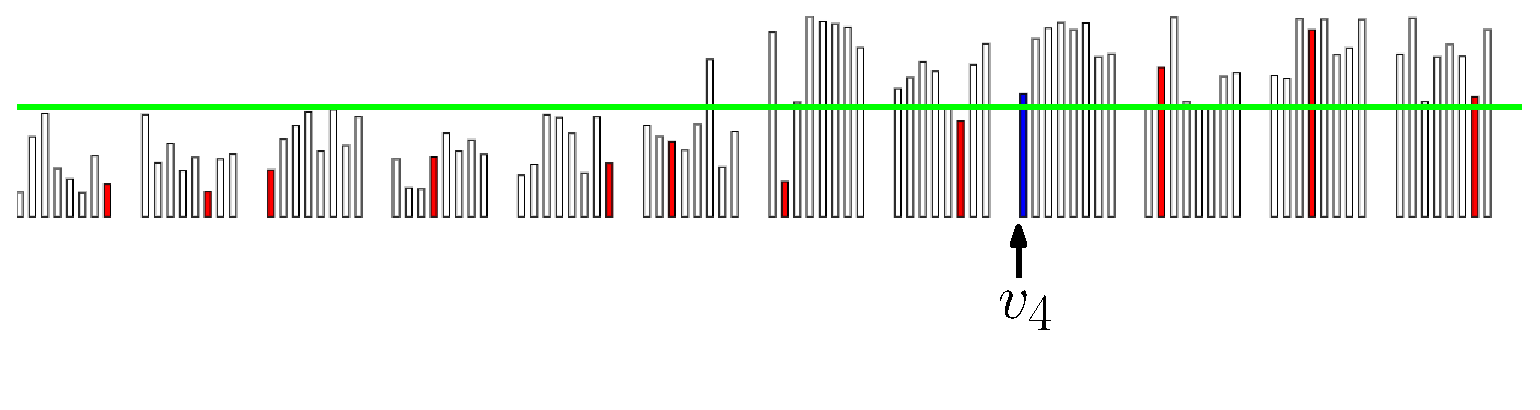
\includegraphics[width=\linewidth]{imgs/smoothedStridingAlgSim/sim35.eps}
  Identify leftmost and rightmost $v_i$. Note that $A[k] \le \text{pivot}$ for all $k < v_{\min}$, and $A[k] > \text{pivot}$ for all $k \ge v_{\max}$.
	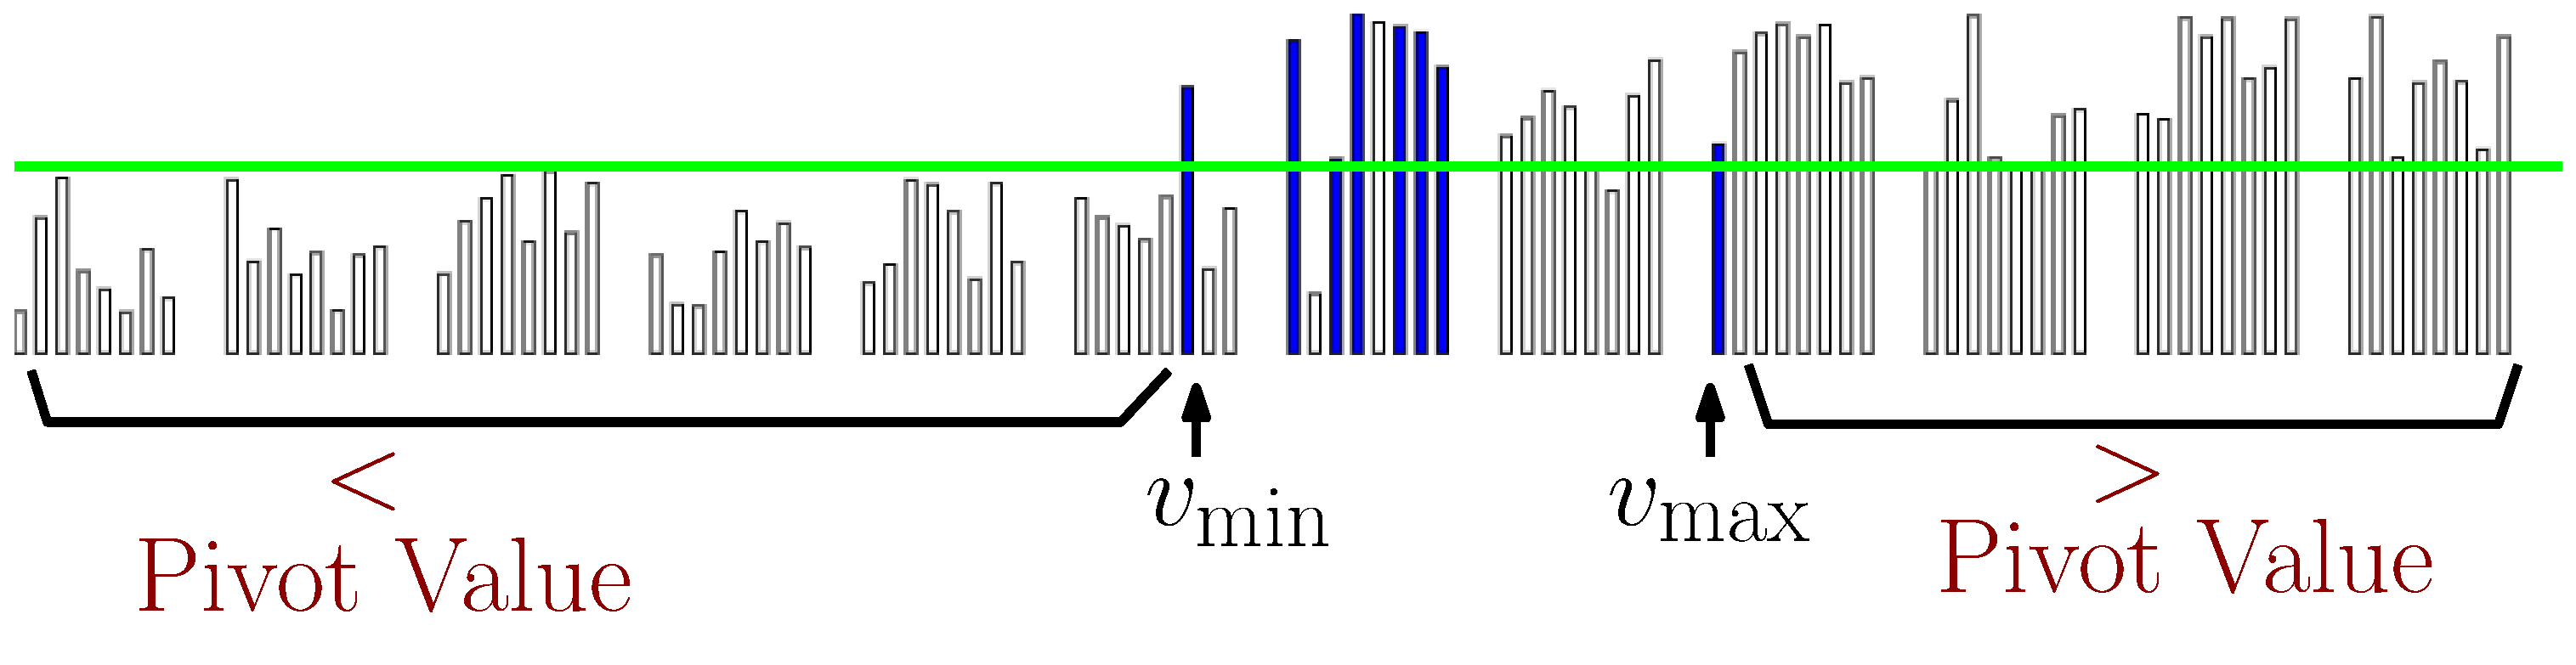
\includegraphics[width=\linewidth]{imgs/smoothedStridingAlgSim/sim4.eps}
	Recursively partition the subarray.\\
  {\color{blue}This step was previously impossible; adding randomization enables this step, which enables our algorithm's low span. }
	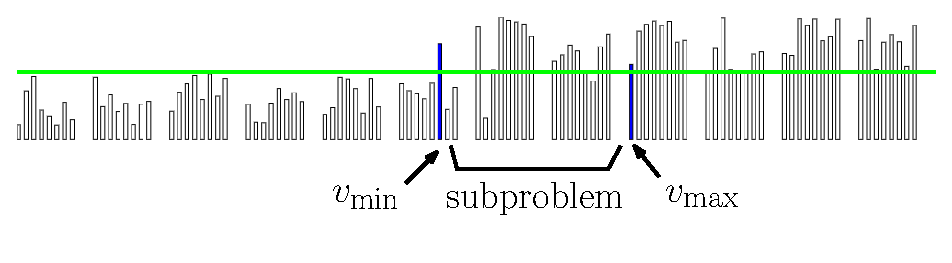
\includegraphics[width=\linewidth]{imgs/smoothedStridingAlgSim/sim45.eps}
\end{block}

\vspace{0.5cm}
\begin{block}{\Huge A Key Challenge}
  \Huge
How do we store the $U_i$'s if they are all random?	\\
\vspace{0.5cm}
Storing which elements make up each $U_i$ takes too much space!\\

\vspace{0.5cm}
\textbf{Strided Algorithm $P_i$.}
\begin{figure}
	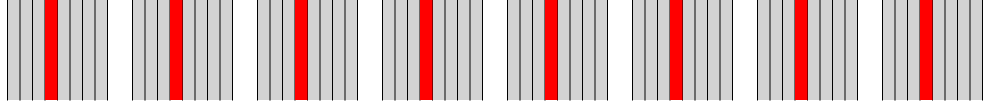
\includegraphics[width=\linewidth]{imgs/stridedAlgHighlighted.png}
\end{figure}
\textbf{Smoothed-Striding Algorithm $U_i$.}
\begin{figure}
	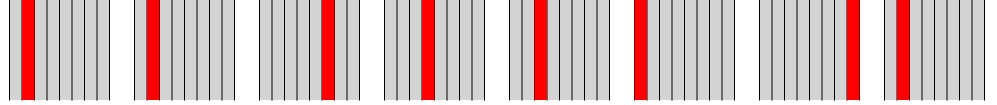
\includegraphics[width=\linewidth]{imgs/smoothedStridingAlgHighlighted.png}
\end{figure}
\end{block}

\vspace{0.5cm}
\begin{block}{\Huge How to Store the groups}
  %TODO fix
  \Huge
	\textbf{Key Insight:} While each $U_i$ does need to contain a random element from each chunk, the $U_i$'s don't need to be \emph{independent}.

	\vspace{0.5cm}
	We store $U_1$, and all other groups are determined by a ``circular shift" of $U_1$ (wraparound within each chunk).
	% Specifically, let $X$ be an array with values chosen uniformly from $\{1,2,\ldots,g\}$. Then the $i$-th element of $U_j$ has index 
	% $$ 1 + ((X[i]+j)\mod g)$$
	\vspace{0.5cm}
	\begin{figure}
		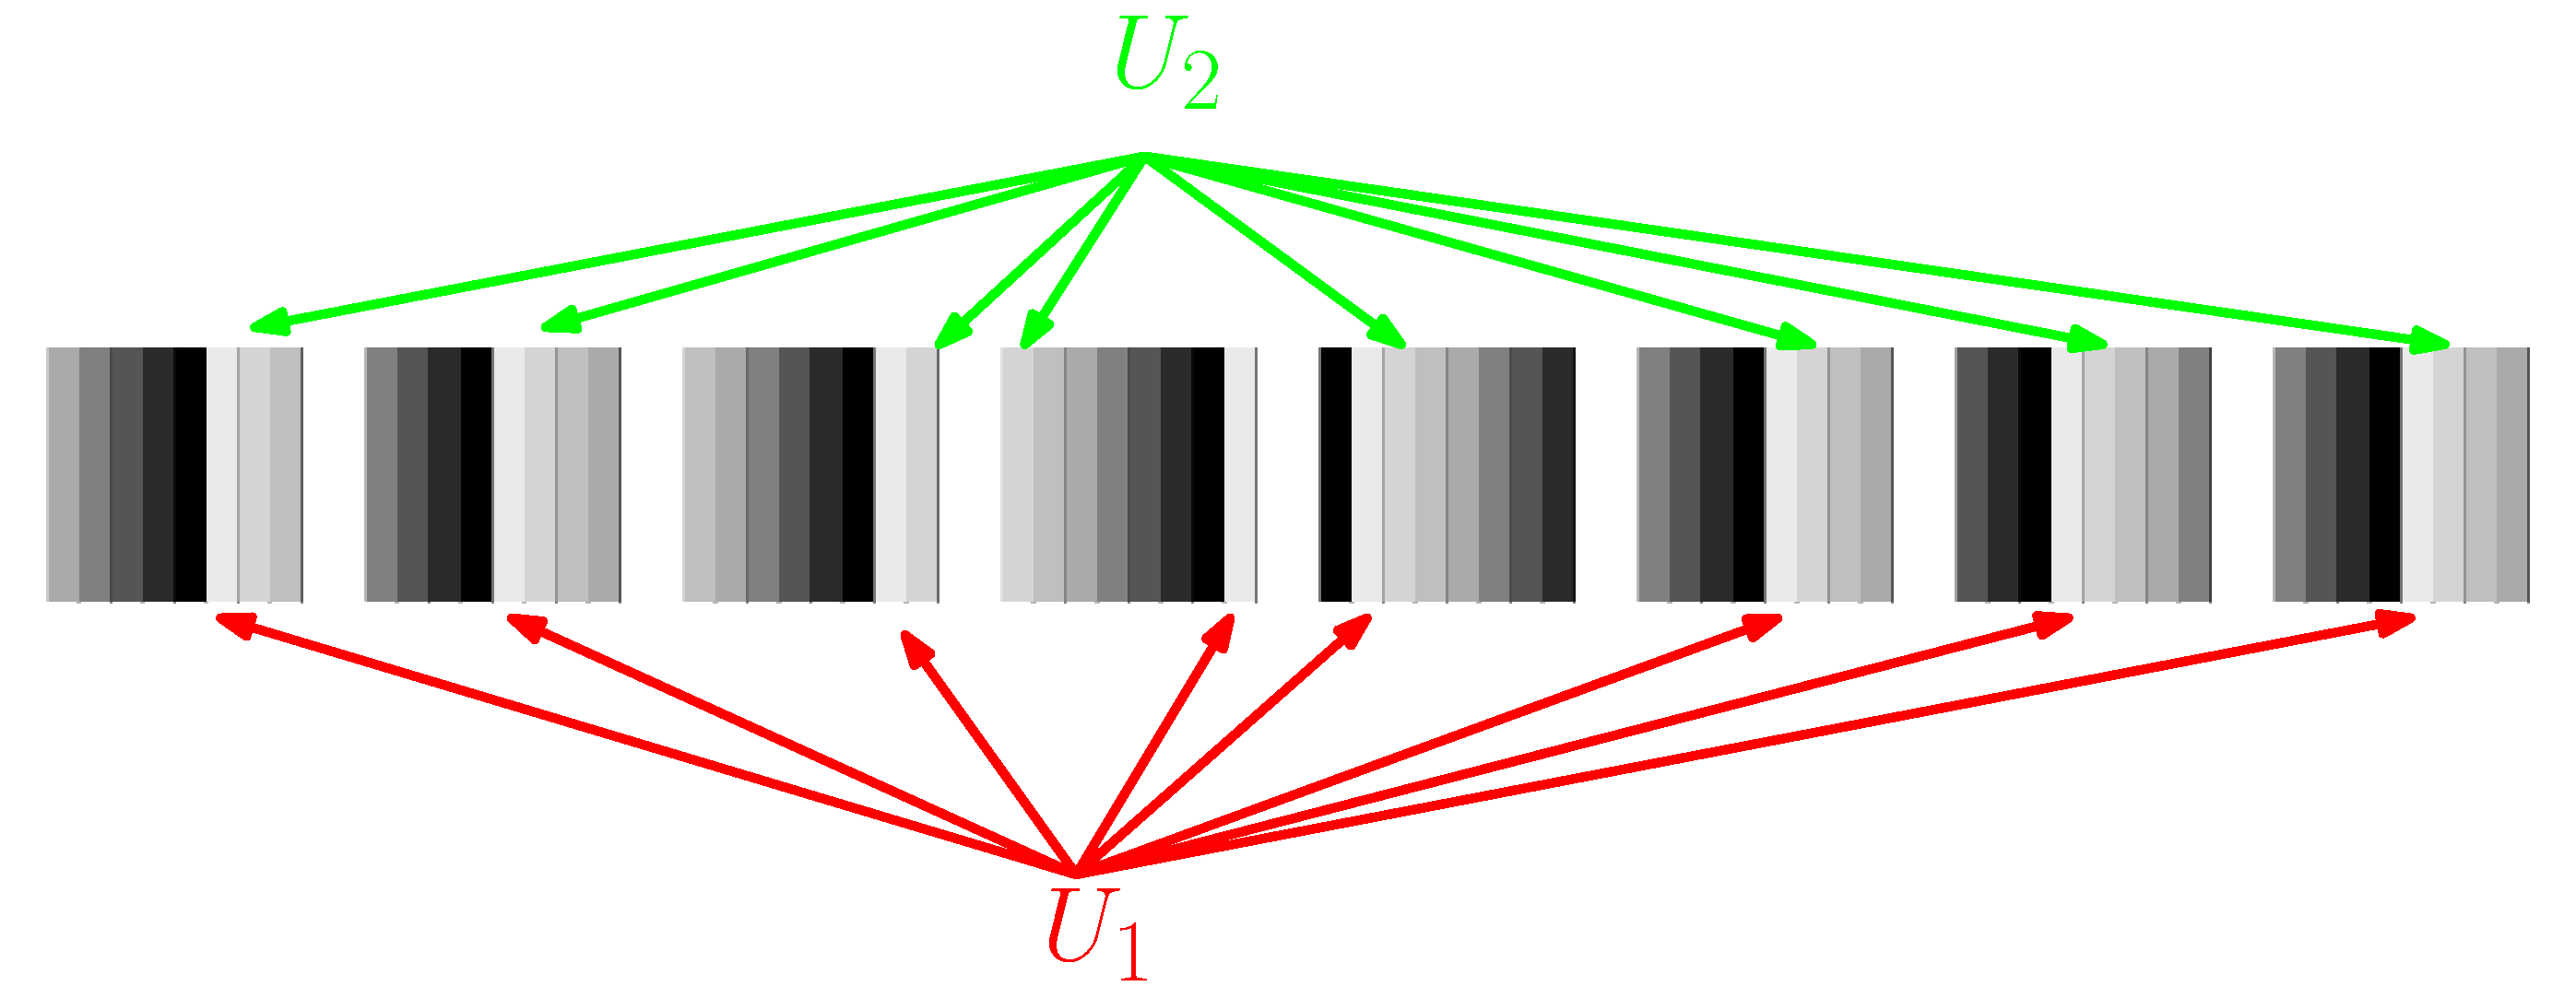
\includegraphics[width=\linewidth]{imgs/blackrainbowAlt.eps}
	\end{figure}	
\end{block}
\end{column}

\begin{column}{0.02\linewidth}
\end{column}

\begin{column}{0.21\linewidth}

  \begin{block}{\Huge Partial Partition Step}
    \Huge
    The \emph{Partial Partition Step} of the Smoothed Striding algorithm guarantees that all elements at index $ i < v_{\min}$ have value $A[i] \le \text{pivot value}$, and all elements at index $i > v_{\max}$ have value $A[i] > \text{pivot value}$. Thus, to completely partition the array a subarray of size $v_{\max} - v_{\min}$ must be partitioned. We prove the following proposition that bounds the size of this subarray:
    
  \textbf{Proposition:\\}
  Let $\epsilon \in (0, 1/2)$ and $\delta \in (0, 1/2)$ such that
  $\epsilon \ge \frac{1}{\poly(n)}$ and $\delta \ge
  \frac{1}{\polylog(n)}$. Suppose $s > \frac{\ln
    (n/\epsilon)}{\delta^2}$. Finally, suppose that each processor has
  a cache of size at least $s + c$ for a sufficiently large constant
  $c$.

  Then the Partial-Partition Algorithm achieves work $O(n)$; achieves
  span $O\left(b \cdot s\right)$; incurs $\frac{s+n}{b} + O(1)$ cache
  misses; and guarantees with probability $1 - \epsilon$ that
  $$v_{\text{max}}-v_{\text{min}} < 4 n \delta.$$
  \end{block}

\begin{block}{\Huge Recursive Strategies}
  \justifying
  % TODO: fix this
  \Huge We propose two algorithms for solving the recursive subproblem: \\
	\begin{itemize}
    \item In the \emph{Hybrid Smoothed Striding Algorithm} we recurse with a (Cache-Inneficient) In-Place Parallel-Partition algorithm, that has span $O(\log n \log \log n)$. With this recursive strategy we achieve span $O(\log n \log \log n)$ overall -- which is within a $\log\log n$ factor of optimal -- and incur fewer than $(n+o(n))/b$ cache misses -- which is optimal up to low order terms-- for appropriate parameter choices, with high probability in $n$.
    \item In the \emph{Recursive Smoothed Striding Algorithm} we recurse with the Smoothed Striding algorithm. {\color{red}This algorithm achieves span $O(\log^2 n)$ which is worse than the other approahc,} but this algorithm {\color{green} has the major benefit of simplicity to implement, while maintaining optimal cache behavior of $(n+o(n))/b$ for appropriate parameter choices, with high probability in $n$}.
	\end{itemize}
\end{block}
\vspace{1cm}

% \begin{block}{\Huge Formal Theoretical Results }
%   \Huge
%   We have the following corrolaries based on the two recursive strategies: 
%   \textbf{Corrolarry: \\}
% Suppose $b \le o(\log \log n)$. Then the Cache-Efficient Full-Partition Algorithm using $\delta = \Theta\big(\sqrt{b/\log\log n}\big)$, achieves work $O(n)$, and with high probability in $n$, achieves span $O(\log n \log\log n)$ and incurs fewer than $(n+o(n))/b$ cache misses.\\

% \textbf{Corrolarry: \\}
%   With high probability in $n$, the Recursive Smoothed Striding Algorithm using parameter $\delta=1/\sqrt{\log n}$:
%   achieves work $O(n)$, attains span $O(b\log^2 n)$, and incurs $n/b \cdot (1 + O(1 / \sqrt{\log n}))$ cache misses. 

% \end{block}
\vspace{1cm}

\begin{block}{\Huge Analysis Overview}
  \justifying
  \Huge
  The proof of our proposition about the Parallel Partition Step proceeds along these lines:
  \begin{itemize}
    \item Let $\mu$ be the faction of elements of the array that are less than the pivot, and $\mu_i$ be the fraction of elements of $U_i$ that are less than the pivot.
    \item All the $\mu_i$ have identical probability distributions, because any given element of the array is equally likely to be assigned to any $U_i$. Hence $\E[\mu_i] = \mu$.
    \item $|U_i| = \polylog n$, so a Hoeffding Bound (Chernoff Bound for random variable on $[0,1]$ instead of on $\{0,1\}$) guarantees that all $U_i$'s
      will have $\mu_i$'s concentrated around $\mu$ with high probability in $n$.
    \item The concentration of $\mu_i$'s induces a concentration of $v_i$'s. 
    \item This guarantees that $v_{\max} - v_{\min}$ is small. 
  \end{itemize}
\end{block}
\vspace{1cm}

\begin{block}{\Huge Pseudocode For the Algorithm}
  \justifying
  \large

\begin{figure}
  % \caption{The Smoothed Striding Algorithm}
  \label{alg:parallelPartition_smoothedStriding}
  \begin{algorithmic}% [1] for line numbers
    \State \textbf{Recall:} 
    \State $A$ is the array to be partitioned, of length $n$. 
    \State We break $A$ into chunks, each consisting of $g$ cache lines of size $b$.
    \State We create $g$ groups $U_1,\ldots, U_g$ that each contain a single cache line from each chunk,
    \State $U_i$'s $j$-th cache line is the $(X[j]+i \bmod g + 1)$-th cache line in the $j$-th chunk of $A$.
    \State

    \Procedure{Get Block Start Index}{$X$, $g$, $b$, $i$, $j$}
      \Comment This procedure returns the index in $A$ of the start of $U_i's$ $j$-th block.
      \State\Return $b\cdot ((X[j] + i \bmod g) +(j-1)\cdot g)+1$
    \EndProcedure
    \State

    \Procedure{ParallelPartition}{$A$, $n$, $g$, $b$}
      \If{$g<2$}
        \State serial partition $A$
      \Else
        \For{$j \in \{1,2,\ldots,n/(gb)\}$}
          \State $X[j] \gets$ a random integer from $[1,g]$ 
        \EndFor

        % \State // \emph{We implement the following parallel for-loop with recursive spawns}
        % \State // \emph{This facilitates computing $v_{min}$, $v_{max}$ without storing $v_y$'s}
        \ForAll{$ i \in \{1,2,\ldots,g\}$ in parallel} \Comment We perform a serial partition on all $U_i$'s in parallel

          \State low $\gets$ GetBlockStartIndex($X$,$g$,$b$,$i$,$1$)
          \Comment low $\gets$ index of the first element in $U_i$
          \State high $\gets$ GetBlockStartIndex($X$,$g$,$b$,$i$,$n/(gb)$) + $b-1$
          \Comment high $\gets$ index of the last element in $U_i$

          \While{low $<$ high} 
            \While{A[low] $\leq$ pivotValue}
              \State low $\gets$ low$+1$
              \If{low $\bmod b \equiv 0$ } 
                \Comment Perform a block increment once low reaches the end of a block
                \State $k \gets $ number of block increments so far (including this one)
                \State low $\gets$ GetBlockStartIndex($X$,$g$,$b$,$i$,$k$)
                \Comment Increase low to start of block $k$ of $G_i$
              \EndIf
            \EndWhile
            \While{A[high] $>$ pivotValue}
              \State high $\gets$ high$-1$
              \If{high $\bmod b \equiv 1$} 
                \Comment Perform a block decrement once high reaches the beginning of a block
                \State $k \gets $ number of block decrements so far (including this one)
                \State $k' \gets n/(gb) - k$
                \State high $\gets$ GetBlockStartIndex($X$, $g$,$b$,$i$,$k'$) $+b-1$
                \Comment Decrease high to end of block $k'$ of $G_i$
              \EndIf
            \EndWhile
            \State Swap $A[\text{low}]$ and $A[\text{high}]$
          \EndWhile
        \EndFor
        \State Recurse on $A[v_{min}],\ldots,A[v_{max}-1]$
      \EndIf
    \EndProcedure
  \end{algorithmic}	
\end{figure}

\end{block}

\end{column}
\begin{column}{0.02\linewidth}
\end{column}


\end{columns}
\end{frame}
\end{document}
